\documentclass[]{article}

\usepackage{float}
\usepackage{graphicx} 

%opening
\title{Encoding and ASCII}
\author{}

\begin{document}

\maketitle


\section{Encoding Basics:} 

\textit{To encode means to use something to represent something else. An encoding is the set of rules with which to convert something from one representation to another.} 

\begin{itemize}
		
\item Computers do not store letters, books or pictures $\rightarrow$ they store bits
\item Bits are the smallest unit of storage on a computer: a 0 or 1
\item \textbf{Encoding} = the mapping between character and code points
\item Encodings use differing number of bits to represent characters:7-bit, 8-bit, 16-bit, etc.
		
\end{itemize}
	
\section{Bits} 
	
\begin{itemize}
\item 8 bits are 1 byte 
\item With n bits, can store $2^n$ patterns
\item Bits represent letters and other characters using a combination of 0 and 1 based on some regulation $\rightarrow$ ASCII
\item Bits are \textbf{case-sensitive}
\item kilobytes, megabytes, gigabytes, etc. are metric aggregations of bytes
	
\end{itemize}

\begin{tabular}{lll}
	& bits  & character \\
	\hline
	& 01100010 & b  \\
	& 01101001 & i \\
	& 01110100 & t \\
	& 01110011 & s \\
\end{tabular}
%

\section{ASCII and Unicode}
\begin{itemize}
	\item ASCII is the original character set/ encoding, only used 7 bits  and was then extended to 8 (ISO-8859-1) $\rightarrow$ $2^8$ = 256 characters 
	\item today \textbf{Unicode} = UTF-8 (MacOS default) or UTF-16 (Windows)
\end{itemize}


\begin{figure}[H]
	\centering
	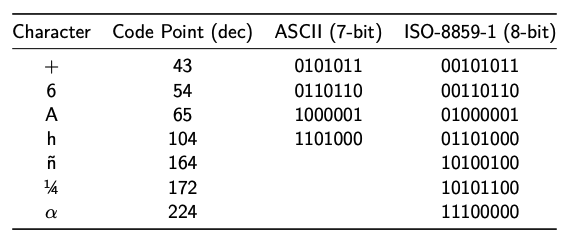
\includegraphics[width=0.7\linewidth]{week04/ASCII table}
	\caption{ASCII Table}
	\label{fig:ascii-table}
\end{figure}


\section{Encoding Issues}
\begin{itemize}
	\item \textbf{Mojibake} = underlying bit sequences translated into the wrong characters $\rightarrow$ wrongly detected encoding of a text file returns gibberish
\end{itemize}
	
	
\end{document}


